\newpage


\section{Fake Lepton Background Estimation}
\label{fk}
%For both the opposite flavor and same flavor analysis, the lepton fake rates are measured as a
%function of the lepton $p_T$ and $\eta$, in a single lepton triggered sample. The test of the method and
%systematic errors are described below.
%\newline
%In the analysis
%the primary source of background from misidentification is W+Jets. QCD multi-jet and hadronic top backgrounds
%are also present at much smaller level. Events in which W bosons are produced in association
%with jets give rise to background to WW events when a jet is misidentified as a lepton. These
%events contain a real lepton and real missing energy from the W decay. With the jet misidentified 
%as a lepton, the W+Jets events have two identified leptons, missing energy, and no other
%significant event characteristics. As a result, the W+Jets events cannot be easily suppressed
%by event selection. This background is particularly important at low $p_T$.
%The estimation of the fake lepton contribution is based on the ``fakeable object'' data-driven
%method and provides a measurement of the yield and the kinematic distributions of fake background. 
%It is a general technique, applicable to any physics analysis in which particle level
%selection criteria are used to suppress background. The method can be used with any number
%of final state particles and is independent of the event selection.
%The fundamental idea of the fakeable objet method is simple: select a control sample of events
%enriched in the background being estimated, and then use an extrapolation factor to relate these
%events to the background in the signal region. The method is data-driven provided the control
%sample is selected in data, and the extrapolation factor is measured with data. For background
%arising from particle misidentification, the extrapolation is done in particle identification space
%($p_T$ and $\eta$ ) of the lepton. The control sample is defined using a looser particle selection criteria
%that are chosen such that the rate of misidentification is increased. The extrapolation factor
%relates background misidentified with this criteria, to background misidentified as passing the
%full particle selection of the signal region.

Events in which a single W boson is produced in association with jets may populate the signal
region when a jet is misidentified as a lepton. 
These events contain a genuine lepton and $p_T^{miss}$ from the W boson decay as well as a second nonprompt lepton from a misidentified jet, likely
rising from a B hadron decay. A similar background arises from semileptonic decays of top
quark pairs, especially in the 1- and 2-jets categories. At a lower rate, multijet production
and fully hadronic top quark pair decays also contribute. These backgrounds are particularly
important for events with low  $p_T$ leptons and low $m_{\ell \ell}$.
The nonprompt lepton background (or fake lepton) is suppressed by the identification and isolation requirements 
imposed on the electrons and muons, while the remaining contribution is estimated
directly from data. A control sample is defined using events in which one lepton passes the
standard lepton identification and isolation criteria and another lepton candidate fails these
criteria but passes a looser selection, resulting in a sample of ``pass-fail'' lepton pairs. 
The pass-fail sample is dominated by nonprompt leptons. The efficiency ($\epsilon_{misID}$) for a jet that satisfies this
looser selection to pass the standard selection is estimated directly from data in an independent
sample dominated by events with nonprompt leptons from multijet processes. 
The contamination of prompt leptons from electroweak processes in such a sample is removed using the
simulation. The uncertainty from this subtraction is propagated to  $\epsilon_{misID}$ . 
The efficiency  $\epsilon_{misID}$  is parameterized as a function of the $p_T$ and $\eta$ of the leptons, 
and is used to weight the events in the pass-fail sample by,  
\begin{equation}
\epsilon_{misID}/(1-\epsilon_{misID}) \; , 
\end{equation}
to obtain the estimated contribution from this background in the signal region. 
The contamination of prompt leptons in the ``pass-fail'' 
sample is corrected for using their probability to pass the standard selection given that they pass
the looser selection, as measured in a Drell-Yan data control sample. 
%The systematic  uncertainty associated with the determination of  $\epsilon_{misID}$  is dominant and arises from the dependence
%of  $\epsilon_{misID}$  on the composition of the jet that is misidentified as a lepton. 
%Its impact is estimated in two independent ways, which are combined to yield a conservative result. 
%First, a closure test performed on simulated W+jets events with  $\epsilon_{misID}$  estimated from simulated QCD multijet
%events provides an overall normalization uncertainty. Second, a shape uncertainty is derived
%by varying the jet $p_T$ threshold in the differential measurement of  $\epsilon_{misID}$  
%in bins of the $\eta$ and $p_T$ of the lepton. 
%The threshold is varied by a quantity that reflects the difference in the fake
%lepton $p_T$ spectrum between W+jets and $t \bar{t}$ events. 
The total uncertainty in  $\epsilon_{misID}$, 
including the statistical precision of the control sample, is about 40\%~\cite{Sirunyan:2018egh}. 
This uncertainty fully covers any data/simulation differences in control regions in which two same-sign leptons are requested.



\section{Lepton Efficiencies from Tag and Probe Method}
\label{TP}
One of the well established data-driven approach for measuring the particle efficiencies is the
so called Tag and Probe method. The Tag and Probe method uses a known mass resonance (e.g. $J/\Psi$, $Z$) to select particles of the desired type, and probe the efficiency of a particular
selection criterion on these particles. In general the “tag” is an object that passes a set of very
tight selection criteria designed to isolate the required particle type. Tags are often referred
to as a “golden” electrons or muons and the fake rate for passing tag selection criteria should
be very small. A generic set of the desired particle type (i.e. with potentially very loose selection 
criteria) known as “probes” is selected by pairing these objects with tags such that the
invariant mass of the combination is consistent with the mass of the resonance. Combinatoric
backgrounds may be eliminated through any of a variety of background subtraction methods
such as fitting, or sideband subtraction. The definition of the probe objects depend on the specifics of the selection criterion being examined. The simple expression to get the efficiency %as a function of $p_T$ and $\eta$ 
is given below:
\begin{equation}
\epsilon=\frac{N_{Pass}^{Probes}}{N_{Pass}^{Probes}+N_{Fail}^{Probes}}
\end{equation}

\subsection*{Electrons} 
The   Tag and Probe is used here to get the identification and isolation efficiency of electrons. In this case, the Tag is a
well identified and isolated electron which also passes an electron trigger. 
Once the Tag electron is selected then another object that pass the kinematic electron selection, Tab.~\ref{IDe}, is searched for. 
The invariant  mass of the Tag and the Probe electron pair is reconstructed and must be in window around the Z boson mass. 
After that, to compute the efficiency, the Probe electron is required  to pass the identification tight working point. 
This procedure is performed for the data and the MC samples. 
Once data and MC efficiencies have been calculated, the electron scale factors are estimated as the ratio among the data and MC efficiencies.  
These scale factors are calculated as a function of $p_T$ and $\eta$ and used to correct the difference in efficiencies between data and MC in the analysis. 
%The Pile-Up reweighting is also applied on MC during the computation of efficiencies. 
%A MC truth matching has also been applied in case of the computation using simulation. 
%In principle, there are two methods to estimate the efficiencies.
%The first one is the \textit{counting method} and the other one is the \textit{fitting method}. 
%The counting method is used when there  are small backgrounds, instead  the fitting method instead when the backgrounds are 
%In order to take into account the effect of DY background in the efficiency estimation,  a fitting method has been used. 
%Tag and Probe pairs are  selected in Z mass window of 60 to 120 GeV.
%If there exist more than one pair then the one whose invariant mass closer to Z pole mass has been selected.
%The efficiencies have been computed as a function of $p_T$ and $\eta$ of electron.
%For signal fitting, MC templates are derived from the simulated sample in the Z mass range 60 to 120 GeV in  $p_T$ and $\eta$ bins.
%The MC Templates are then smeared using Gaussian function. For the background fitting a function, that is combination of
%an exponential function and an error function, has been used.
%The exponential decay distribution becomes
%active at high mass beyond the Z peak and the error function takes over at low masses due to
%threshold effect.
%A fit examples for all $p_T$ bins is shown in Fig.~\ref{ac}
%\begin{figure}
%\centering
%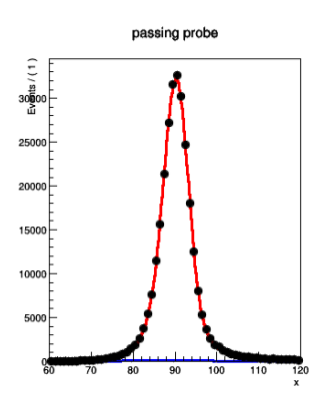
\includegraphics[scale= 0.5]{tpe}
%\caption{Fits for $p_T$ bin (35-50) GeV and $\eta$ in (-2.5,-2.0) bin.}
%\label{ac}
%\end{figure}

The electron efficiency is about 95\%, on the trigger plateau. 


\subsection*{Muons} 
The muon identification and isolation efficiency is also studied and compared to the prediction of MC in order
to understand if a correction is needed. The muon efficiency is obtained as
\begin{equation}
\epsilon_{\mu} = \epsilon_{TRK} \times \epsilon_{Tight} \times \epsilon_{ISO \; Tight} \; ,
\end{equation}
\newline
where $ \epsilon_{TRK}$ is the tracker  muon efficiency.  
The $ \epsilon_{Tight} $ is muon efficiency
under the assumption that the muon passes the kinematic selections summarized in  Tab.~\ref{IDm}.
The $\epsilon_{ISO \; Tight}$ is the efficiency of the isolation criteria under the assumption that the muon passes the same selection.
The $\epsilon_{Tight}$ and $ \epsilon_{ISO \; Tight}$ are determined  using the Tag and Probe method. 
The Tag muon is obtained by applying  the kinematic selections  and   the isolated muon trigger  with $p_T^{\mu}>20$ GeV.
The Probe muon  is requested to pass the kinematic selection and the isolation criteria.
%After that it is checked if the Probe muon is matched to the muon trigger. 
%In general the efficiencies are relatively high due to the lower cut on $p_T$ and the looser cut on
%isolation %in the double lepton trigger compared to single muon trigger. 
The efficiency value on the plateau is around 93\%-99\%.



\newpage

\section{Systematic uncertainties}\label{sec:systematics}
Systematic uncertainties are introduced as nuisance parameters in the fit and can affect the
normalization and the shape of the different contributions.\\
Systematic uncertainties are represented by individual nuisance parameters with log-normal or
modified shape distributions. These uncertainties affectt the overall normalization of the signal and
backgrounds as well as the shape of the predictions across the distribution of the observables.
Correlations between systematic uncertainties in different categories and final states are taken
into account. Statistical uncertainties from MC simulated events are also considered.
Systematic uncertainties play an especially important role in this analysis where
no strong mass peak is expected due to the presence of undetected neutrinos in the final state.
Below, it is describe in detail the sources and the quantities of systematics for this analysis and their
effects on the signal and background processes. A list of the most important background uncertainties is given is also introduced.


\subsection*{Background normalization uncertainties}
One of the most important sources of systematic uncertainty is the normalization of the backgrounds that are estimated on data control samples whenever is possible. The signal extraction is performed subtracting the estimated backgrounds to the event counts in data. The amount of uncertainty depends on the considered background:
\begin{itemize}
\item  jet-induced background: normalization and kinematic shapes are derived from a
data control region and both normalization and shape systematic uncertainties are
considered. A conservative 30$\%$ uncertainty on the fake rate is assumed correlated across the different analysis regions. The contribution to the uncertainty in the signal region due to the limited electron statistics in the background enriched control regions is about 10\%, while the contribution due
to the limited muon statistics is 3\%. 
\item WW background: The normalization of the WW background is performed independently in each jet multiplicity. 
A WW electroweak (VBS) sample is used in addition to the standard WW sample in
the phase spaces with at least two jets, where its contribution becomes non negligible.
The uncertainty in the cross section for this process is evaluated using the variations
of the renormalization and factorization QCD scales, as well as the PDF variations,
and amounts to 11\%.
\item $\bar{t}t$ and tW backgrounds: top events are estimated with b-tagging in data control regions. 
The top background enriched control regions are defined as additional categories in the fit while the kinematic shapes are taken 
from the simulation corrected for the b-tagging scale factors. 
The top normalization is correlated between the top control region and the high mass signal categories 
separately in  different jet multiplicities, and these normalizations are left unconstrained. 
A nuisance parameter is added to take into account the effect of the parton shower uncertainty on the top background.

\item Drell-Yan background: The Drell-Yan background enters the different flavor analysis via the leptonic decays of the $\tau$ leptons from $Z \gamma^* \to \tau \tau$. In the different flavor
analyses the normalization of these background is constrained using a dedicated control region in each jet bin category. 
A dedicated nuisances for MET reweighting in DY control region is introduced in same flavour analysis. It is evaluate separately for ee and $\mu \mu$ categories. 
The uncertainty is quoted as the envelope of the the maximum and minimum result of the linear fit.

\item $W \gamma^*$ background: The kinematic shape of this background is predicted by simulation, normalized to its data-driven estimate, and constrained within the respective
uncertainty, which is 25\%.
\item WZ : The kinematic shapes of this backgrounds are predicted by simulation and
normalized to their theoretical predictions in the different and same flavour analysis.

\item $ Z \gamma^*$  : The kinematic shapes of this backgrounds are predicted by simulation and
normalized to their theoretical predictions in the different and same flavor analysis.

\item ZZ: The kinematic shapes of this backgrounds are predicted by simulation and normalized to their theoretical predictions in the different and same flavor analysis.

\end{itemize}


\subsection*{Experimental uncertainties}
Effects from experimental uncertainties are studied by applying a scaling and/or smearing of
certain variables of the physics objects, followed by a subsequent recalculation of all the correlated variables. This is done for MC simulation, to account for possible systematic mismeasurements of the data. All experimental sources except luminosity are treated both as normalization and shape uncertainties. For background with a data-driven normalization estimation,
the shape uncertainty is considered only. 
The following experimental systematic sources have been taken into account.

\begin{itemize}
\item Luminosity: The uncertainty determined by the CMS luminosity monitoring is 2.3\% for 13 TeV data~\cite{CMS-PAS-LUM-17-001}.
\item Lepton trigger systematics: Lepton trigger systematics are of the order of less than 1\%. 
These uncertainties are computed by varying the tag selection
as well as the Z window in the tag and probe method used to compute the corresponding scale factors.
\item Lepton reconstruction and identification efficiency:
The lepton reconstruction and identification efficiencies are measured with the tag
and probe method in data. To correct for the difference in the lepton identification
efficiencies between data and MC, data/MC scale factors dependent on \pt and $\eta$ are
applied to the MC. The resulting uncertainty in the signal region is  1\% for electrons
and 2\% for muon.
\item Muon momentum and electron energy scale:  Uncertainties on both the scale and resolution individually amount to  0.6-1\% for electrons 
and  0.2\% for muons. 

\item MET mismodelling: The MET determination is affected by possible mismeasurements of the particles in the collision of interest, 
as well as by additional contributions from the pile-up interactions. The effect of the missing transverse momentum resolution on the event selection is studied by propagating each component of the MET uncertainty to the absolute value and direction of MET.

\item Jet energy scale (JES) uncertainties: this uncertainty is estimated 
applying the official jet uncertainties on the JES  and computeing the variation of the selection efficiency. JES uncertainty affects the
rates in the signal region at the level of  10\%.

\item b-jet misidentification modelling: the uncertainties on the selection of non-b jets is taken into account by looking at
the b-jet misidentification efficiency. The uncertainties on these scale factors are of the
order of a few percent.
\end{itemize}


\subsection*{ Theoretical uncertainties}
The uncertainties due to the precision of theoretical calculation are listed below: 
\begin{itemize}
\item PDF and higher-order corrections (renormalization and factorization scale): PDF
uncertainties and the missing knowledge on higher-order corrections are evaluated by
means of scale variations. They directly affect the cross section, as well as the acceptance
of a simulated process. The uncertainties that arise from using different PDF sets
were obtained by reweighting events to the different PDF sets.

\item Underlying event and parton shower modelling: The underlying event (UE) and
parton shower (PS) modelling uncertainties are estimated by comparing samples
obtained with different parton showers (Pythia vs Herwig) and UE tunes

\item Single top tW and tt ratio: The ratio between the single top and top pair cross section
is varied by the uncertainty on the ratio between their cross sections, estimated considering scale variations,

\item QCD and PDF scales for the signal samples at different masses have been included. These uncertainties are taken from the Yellow Report 3~\cite{Heinemeyer:2013tqa}.  The effect of QCD and PDF scale uncertainties on the analysis selection has aslo been taken into account.


\item The categorization of events based on jet multiplicity introduces additional uncertainties related to higher order corrections. These uncertainties are associated to the gluon-gluon fusion production mode and are evaluated independently following the recipe described in~\cite{Boughezal:2013oha} and are 5.6\% for the 0-jet and  13\% for the 1-jet and 20\% for the 2-jet and VBF categories.

\end{itemize}



